 \documentclass[%
    corpo=11pt,
    twoside,
%    stile=classica,
    oldstyle,
%    autoretitolo,
    tipotesi=magistrale,
    greek,
    evenboxes,
    english,
]{toptesi}


\usepackage[utf8]{inputenc}% codifica d'entrata
\usepackage[T1]{fontenc}%    codifica dei font
\usepackage{lmodern}%        scelta dei font
\usepackage[utf8]{inputenc}


\usepackage{hyperref}
\usepackage{import}
\hypersetup{%
    pdfpagemode={UseOutlines},
    bookmarksopen,
    pdfstartview={FitH},
    colorlinks,
    linkcolor={blue},
    citecolor={blue},
    urlcolor={blue}
  }




\begin{document}\errorcontextlines=9
%%%%%%% Questi comandi è meglio metterli dentro l'ambiente
%%%%%%% ThesisTitlePage con o senza asterisco, oppure in un file di
%%%%%%% configurazione personale. Si veda la documentazione
%%%%%%% inglese o italiana.
%%%%%%% Comunque i presenti comandi servono per comporre la
%%%%%%% tesi con i moduli di estensione standard del pacchetto
%%%%%%% TOPtesi.

\begin{ThesisTitlePage}
% Per cambiare la dicitura sopra la lista dei laureandi decommentare
% la riga seguente, cambiando le 4 parole in modo consistente
%
\TitoloListaCandidati{Studente,Studenti,Studentessa,Studentesse}
%
\ateneo{Politecnico di Torino}
%
% Non tutte le università hanno un nome proprio
%\nomeateneo{}
%
\struttura[III]{Matematica, Fisica e~Scienze Naturali}
%\Materia{Remote sensing}
\titolo{}% per la laurea quinquennale e il dottorato

%
%%%%%%% Corso degli studi
\corsodilaurea{Electronic Engineering}% per la laurea
%%%%%%% L'eventuale numero di matricola va fra parentesi quadre
%\show\Candidato
%\def\Candidato{Studente}
%\show\Candidato
\candidato{Vito Luca \textsc{Guglielmi}}[s265044] 
%\secondocandidato{Evangelista \textsc{Torricelli}}[123457]

%%%%%%% Relatori o supervisori
%
    \relatore{prof.~Luciano Lavagno}
    \secondorelatore{prof.~ Francesc Moll Echeto}
    \terzorelatore{dott.~Oscar Palomar}
% 
%%%%%%% Per mettere altri relatori consultare toptesi-it.pdf

%%%%%%% Tutore
%\tutoreaziendale{}
\NomeTutoreAziendale{Barcelona Supercomputing Center}

%%%%%%% Seduta dell'esame
%\sedutadilaurea{Agosto 1615}
%%%%%%%% oppure:
\sedutadilaurea{\textsc{Anno~accademico} 2019-2020}% 

%%%%%%% Logo della sede
\logosede{LOGO.png}% 
\end{ThesisTitlePage}


%%%%%%% Per cambiare l'offset per la rilegatura;
%%%%%%% meno offset c'e', meglio e'
%\setbindingcorrection{3mm}

{\begin{dedica}
    \normalsize{Alla mia famiglia}
\end{dedica}

\newpage
\english
\summary
\english

This thesis was developed while working at Barcelona Supercomputing Center, a research center specialized in High Performance Computing and investigation in many fields, such as cloud computing, bioinformatics, material science and more.\\


Taking part to European Processor Initiative (EPI) project, the whole thesis aims to perform the verification process on a Vector Processing Unit.
The implemented Vector Processing Unit is based on the RISC-V V-Extension, which is a set of specifications defining the Instructions Set Architecture (ISA) of a vector core. The V-Extension is currently on develop by the RISC-V foundation. This manuscript will refer to the versions 0.7.1.\\

The   first  chapter consist of an introduction of the needed concepts and of the context in which this thesis is been developed.\\

Then, in the second chapter, all the techniques used to verify functionally and formally this VPU are discussed.\\

All the results, such as found bugs or created material, are displayed in the third chapter. Moreover, analysing these results, the efficacy of the techniques used is evaluated. It is shown how formal and functional tools can be used to find bugs or to better define specification. \\

In the last chapter, it is possible to conclude that the techniques  adopted produced the expected results showing significant improvements in the verification effort.








\bigskip



\tableofcontents
\clearpage
\mainmatter


\chapter{Introduction}
This thesis is based on part of the EPI-project, developed at Barcelona Supercomputing Center, in particular on the V-Extension implementation.
In this Chapter there will be presented and discussed all the RISC-V and V-Extension concepts, but they will be not covered all the topics regarding the RISC-V ISA or all the extensions, as they are not always relevant to the project.\\
Starting from the Concepts there will be also an explaination on the context of the project, so the real implementation and application of the ISA specifications.
In particular there will be a exposition of Verification concepts and on the UVM structure, filled by the details useful to understand the work done.



\section{Concepts}
\subsection{RISC-V}
RISC-V is an open, extensible and free instruction set architecture (ISA). It was originally designed to support computer architecture research and education\cite{RISC-V-Instruction-Set-Manual}.\\
The project began at the Berkley, University of California in 2010, and then in 2011 was published the first ISA User Manual. After that there was the first tapeout of a RISC-V chip in 28nm FDSOI donated by STMicroelectronics.\\

The RISC-V ISA is implemented as a base integer ISA, but it is modular and so supports  variable-length instruction encodings.\\
This ISA is provided under open source licenses, and it is gaining a lot of popularity due to its open nature. \\
Mainly there are two primary base integer variants, RV32I and RV64I, which provide 32-bit or 64-bit user-level address spaces respectively.\\

RISC-V is designed to have good customization and so it's provided with the possibility to be extended, but the base integer instructions cannot be redefined.\\
There are two kinds of extensions:
\textit{standard} and \textit{non-standard}.
\begin{itemize}
    \item The \textit{standard} ones need to be compatible with all the other standards and also they should aim to be generally useful.
    \item The \textit{non-standard} ones can be highly specialized in some task and so can be in conflict with other extensions.
\end{itemize}

For general development some standard extensions are predefined:
\begin{itemize}
    \item "\textbf{I}" is the base integer extension and contains integer computational instructions, integer loads, integer stores, and control-flow instructions. It is mandatory for all RISC-V implementations.
    
    \item "\textbf{M}" is the standard integer multiplication and division extension, it allows to multiply and divide the values held in the integer registers.
    
    \item "\textbf{A}" is the standard atomic instruction extension. For inter-processor synchronization is useful to have atomic instructions so with this extension is possible to read, modify, and write memory atomically . 
    
    \item "\textbf{F}" is the standard single-precision floating-point extension. It adds floating-point registers, single-precision computational instructions, and single-precision loads and stores. 
    
    \item "\textbf{D}" The standard double-precision floating-point extension. It is useful when the F extension is not enough, so expands it and adds double-precision computational instructions, loads, and stores.
    
    \item "\textbf{G}" is the denotation for an integer base plus these four standard extensions (“IMAFD”).
\end{itemize}


The design philosophy of the RISC-V projects is based on modularity: the base ISA will not change over time, but new extensions will be available and new feature will be added. This is useful because is very difficult to find general useful extension beyond the ones already exist. So it wouldn't be convenient to constantly add new features to the base ISA and then have to keep track of that.\\
In Figure \ref{riscv-base-instruction-formats} it is possible to see how the base instruction are composed.

\begin{figure}[H]
    \centering
    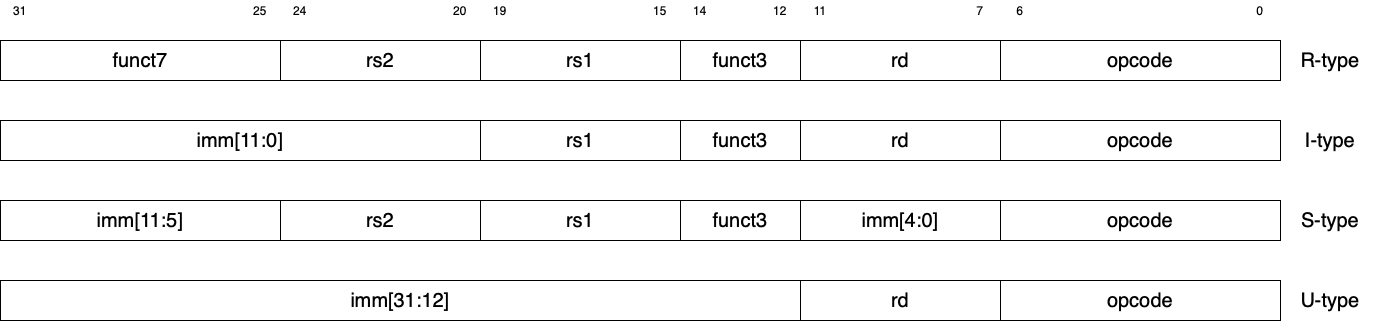
\includegraphics[scale = 0.27]{Chapter_1/img/riscv-base-instruction-formats.png}
    \caption{RISC-V base instruction formats. \cite{RISC-V-Instruction-Set-Manual}}
    \label{riscv-base-instruction-formats}
\end{figure}

It is important to notice that RISC-V is a load-store architecture, this means only load and store operations can have access to the memory.\\
It is a very convenient organization, because it reduces the average time-per-operation and guarantees a good functioning of the pipelined structure.\\

It also supports signed byte and half word loads, which is very useful when  working with signed byte and half word data types.

In Figure \ref{riscv-load-store} it is possible to see how the load-store instructions are composed, and that the LOAD is a I-type op and the STORE is an S-type op.

\begin{figure}[H]
    \centering
    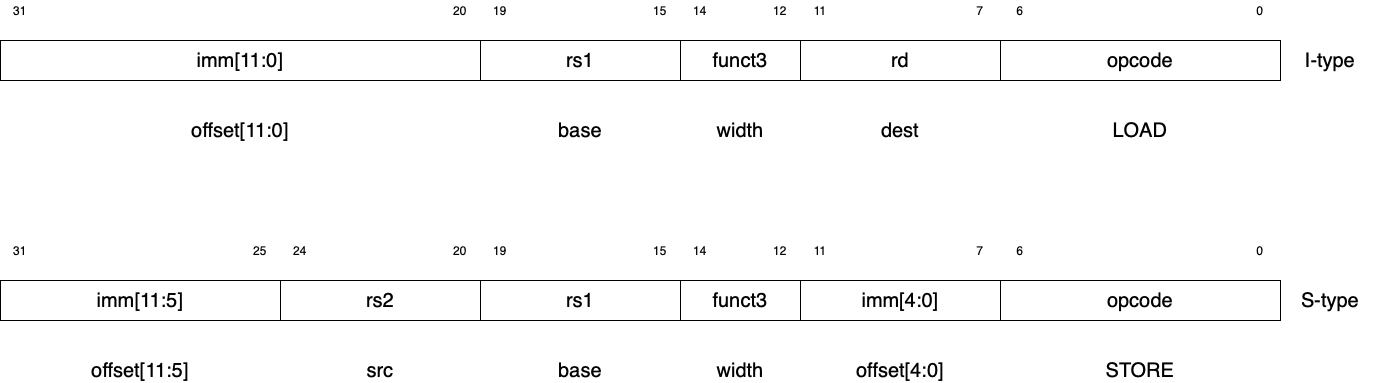
\includegraphics[scale = 0.27]{Chapter_1/img/riscv-load-store.png}
    \caption{RISC-V load/store instruction formats. \cite{RISC-V-Instruction-Set-Manual}}
    \label{riscv-load-store}
\end{figure}


\subsection{Parallel architectures, Vectors and RISC-V V-Extension}
In the last years the parallel architecture are gaining inertia on the processors field. This is happening because the real world has parallel behaviour and so the hardware we use to compute simulations and calculus needs to be.\cite{Parallel-Computing}\\
But why now and not before?\\
In the past, parallel computing efforts have shown promise and gathered investment, but in the end, uniprocessor computing always prevailed, what is different now?\\
Well, most of the paradigms that led to the unicore decision are now changing quickly as the technology changes its needs.\\
As the technology scales down to the nanometers, the power consumption and the energy consumption are becoming a problem, instead the cost of a single transistor is significantly lower.\\

But the multicore solution still doesn't meet the conformity for old binaries compilations and it could be difficult to program. So the solution of a parallel architecture with "manycores" seems to be the right one.\\

For this reason the vectors are useful. They allow to compute data in a parallel way, without having multicore programming logic.\\
A classic example are the VPU (Vector Processing Units) working with SIMD (single instruction multiple data).\\

A famous example of a vector architecture is the Cray-1. It was presented in 1975, and was a load/store architecture, as seen before.
It was designed for Supercomputing and the major feature was to have also a scalar mode. This because the vector computation is not always useful.\\

As it is possible to see in Figure \ref{Multithreading} with standard multithreading there will always be some empty thread along with the running ones. This lowes the efficiency.
\begin{figure}[H]
    \centering
    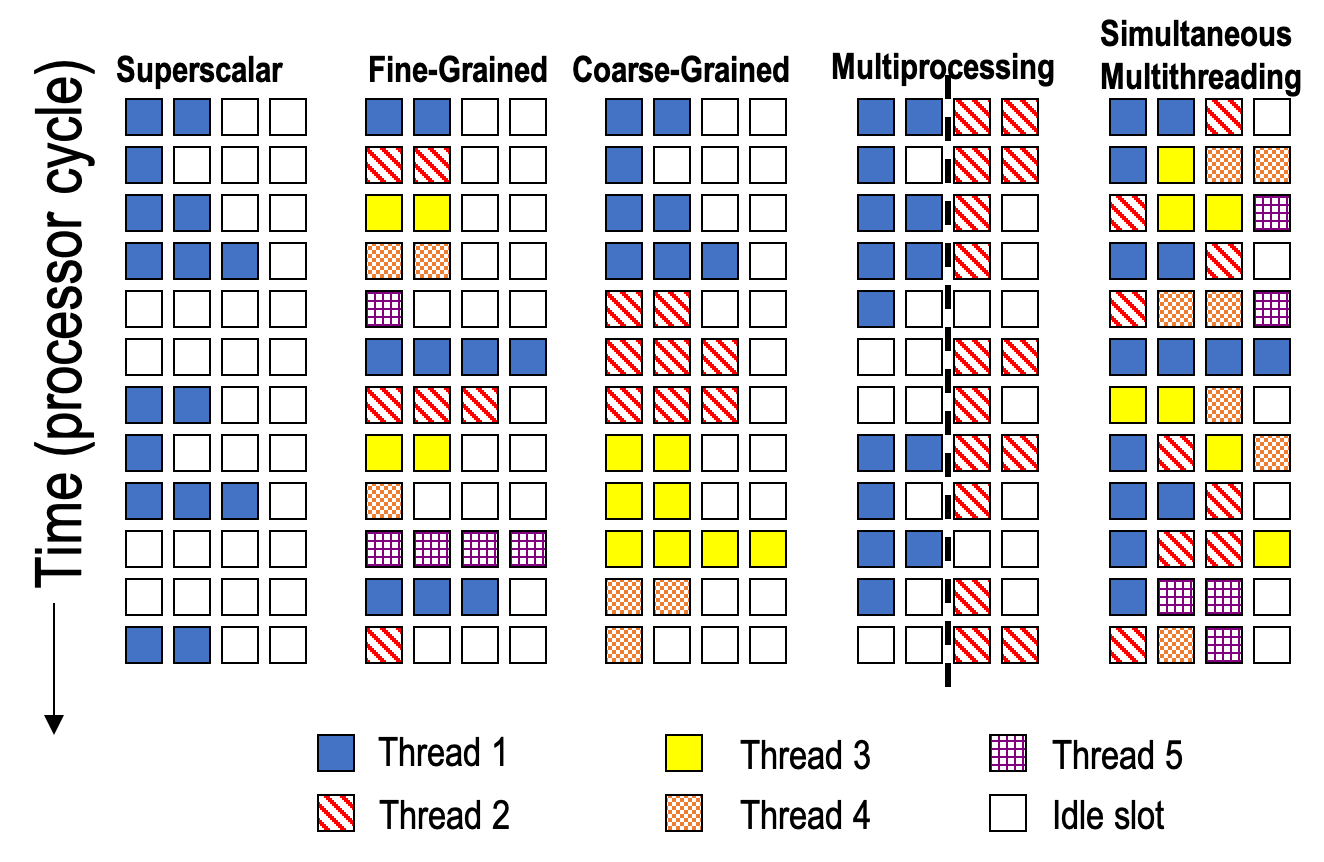
\includegraphics[scale = 0.4]{Chapter_1/img/multithreading.png}
    \caption{Multithreading Processor Clock Time usage  \cite{L15-Krste}}
    \label{Multithreading}
\end{figure}

Indeed the major advantage with the Vector computation is the condensation of the processor usage. 
So the usage will not be distributed as for standard multithreading processors, but it will have full usage for some cycles and zero usage for others\cite{L15-Krste}.\\

But of course there is a drawback, in particular the Latency. In vector computing there are always some dead cycles, but this also allows to increase the efficiency with modern low-power techniques, if it is possible to decrease the energy usage during the dead time.
The pipeline is represented in Figure \ref{Vector-Latency} and the final Clock Tima usage is represented in Figure \ref{Vectoring}.

\begin{figure}[H]
    \centering
    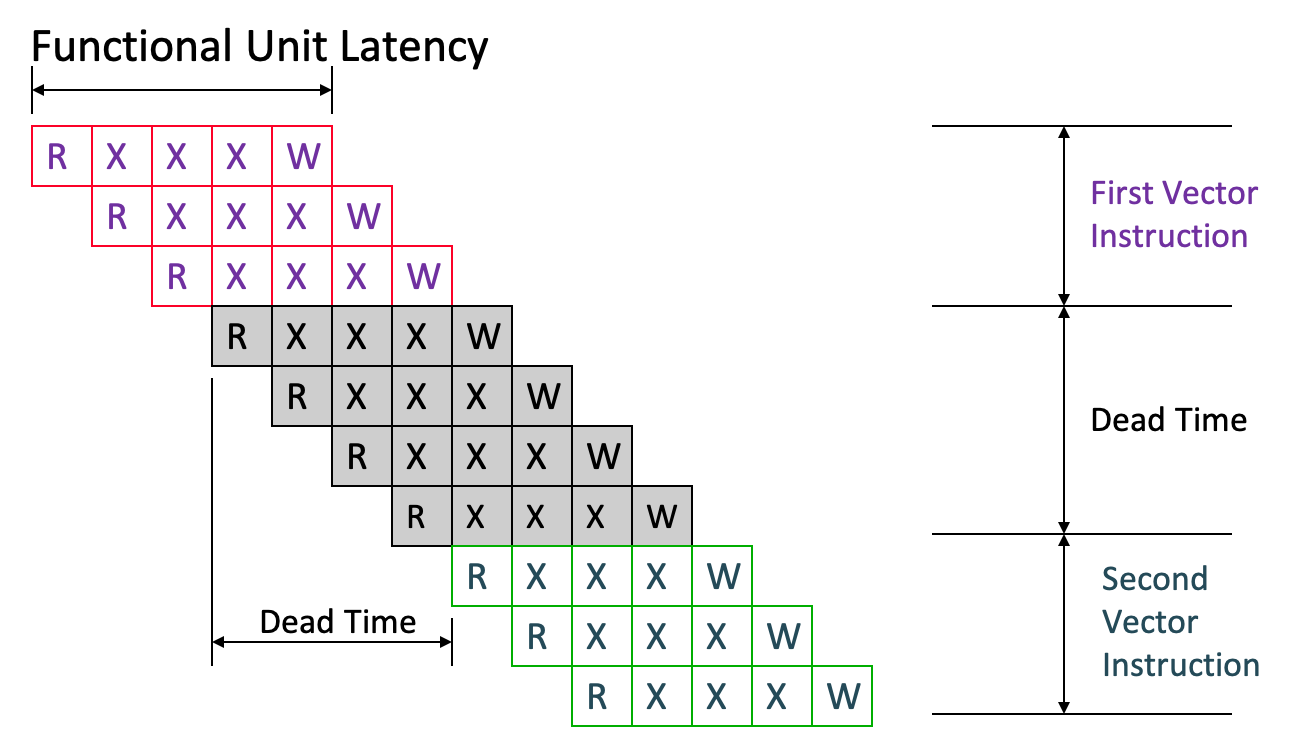
\includegraphics[scale = 0.4]{Chapter_1/img/vectoring.png}
    \caption{Latency penalty on vector processing units \cite{L15-Krste}}
    \label{Vector-Latency}
\end{figure}

\begin{figure}[H]
    \centering
    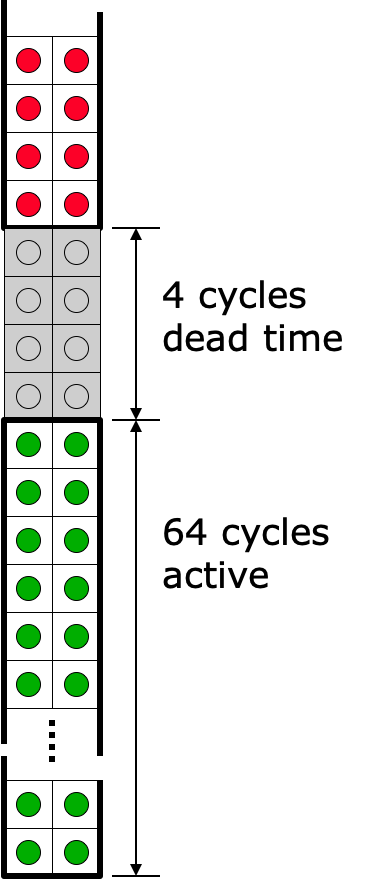
\includegraphics[scale = 0.4]{Chapter_1/img/vectoring_2.png}
    \caption{Vector Processor Clock Time usage \cite{L15-Krste}}
    \label{Vectoring}
\end{figure}
The RISC-V solution is V-Extension (V stands for Vector), and is in current development, in this thesis the reference will be the V-Extension 0.7.1.

The vector extension adds 32 vector registers, and five unprivileged CSRs (vstart, vxsat, vxrm, vtype, vl) to a base scalar RISC-V ISA\cite{riscv-v-specs}.
There are also 8 vector predicate registers (vp0-vp7). The CSRs vectors define the configurations.

\begin{table}[H]
    \centering
    \begin{tabular}{|l|l|l|l|}
        \hline
        Address & Privilege & Name   & Description               \\ \hline
        0x008   & URW       & vstart & Vector start position     \\ \hline
        0x009   & URW       & vxsat  & Fixed-point Saturate Flag \\ \hline
        0x00A   & URW       & vxrm   & Fixed-Point Rounding Mode \\ \hline
        0xC20   & URO       & vl     & Vector length             \\ \hline
        0xC21   & URO       & vtype  & Vector data type register \\ \hline
    \end{tabular}
    \caption{RISC-V's CSRs}
    \label{CSRs}
\end{table}

Based on the base scalar ISA and on the extensions implemented the datatypes and operations supported by the V extension change and they can be 16-bit, 32-bit, 64-bit, and 128-bit floating-point types or fixed-point types (F16, F32, F64, and F128, or X8, X16, X32, X64, and X128 respectively) \cite{riscv-v-specs}.\\


The vector unit must be configured before use. 
The active vector length is held in the CSR vl, which can only hold values between 0 and MVL inclusive.
The active vector length is usually written with the setvl instruction.\\

Other than the base instruction we can expect from a Vector Architecture (as a move, add, xor and so on) it is possible to find some useful operations related to the nature of the vector calculus\cite{riscv-v-specs}:
\begin{itemize}
    \item \textbf{vectorial load/store}: those can strided or indexed. The strided ones index the elements referring to a starting one and then adding (or subtracting) a certain stride. This kind of load/store is very fast, in particular in some special cases (as unit-strided or some optimized power of 2).\\
    The elements into the indexed ones are basically pointed with an index. This process really slows down the operation but allows to select directly the elements.
    
    \item \textbf{widening/narrowing}: those operation are used to increase or decrease the size of the vector's contents, in fact they are very useful when performing operations that need to increase the result size (as example a multiplication between to integer at 32 bit needs to have 64 bit to not loose information). There are also few operations that require the inverse resizing, so the narrowing.
    
    \item \textbf{gather}: those are very particular operations and very useful when manipulating vectors. They allow to index a vector using another vector as index. In this way various patterns are possible.
    
    \item \textbf{reduction}: finally the reduction can perform an operation between a scalar and a vector and give as result a scalar (an easy example could be to calculate the maximum value between all the value contained in a vector and one scalar, the result would either be one of the element of the vector or the scalar).
    
\end{itemize}


Finally all those operations can be \textit{masked}. The masking is a common operation when there is branching or when complex patterns emerge.
Normally one bit of the mask represent a whole work or byte into the vector. Then an AND op is performed to have the final result. 

\subsection{Verification}
As the technology scales down, the design complexity explodes. 
Very small form factor have conflicting requirements for high performance, low-power and area constraints. 
This lead to a complex design and to elevate the costs of it.\\

It is possible to see in Figure \ref{verification-tecnology} how the cost for verification increases drastically with the lowering of the technology node.


\begin{figure}[H]
    \centering
    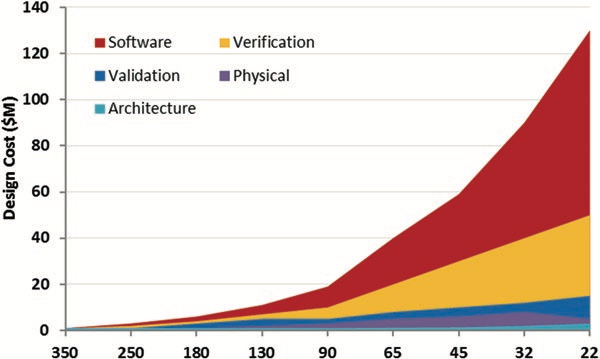
\includegraphics[scale = 0.6]{Chapter_1/img/verification-tecnology.png}
    \caption{Verification cost vs technology node \cite{verification-book-2018}}
    \label{verification-tecnology}
\end{figure}

the verification is responsible to make sure the design is in track with the specification, so as the design complexity increases so does the verification.\\

This is of course an issue for the time-to-market. 
In particular functional design verification takes 40–50\% of the project resources. In other words, increase the productivity of functional design verification and shorten the design / simulate / debug / cover loop is an essential task \cite{verification-book-2018}.\\

Also the compounded complexity grows faster that the compounded productivity. This gap only means the verification needs to be faster and so need to implement more techniques.
It is possible to see a study on the complexity/productivity gap in Figure \ref{complexity-gap}
\begin{figure}[H]
    \centering
    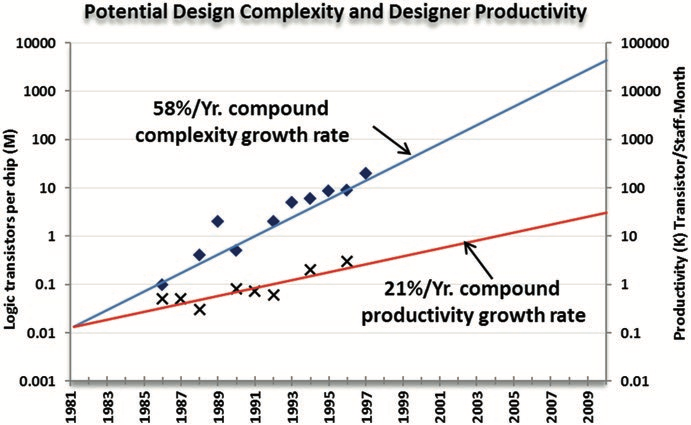
\includegraphics[scale = 0.5]{Chapter_1/img/complexity-gap.png}
    \caption{The gap between the complexity and the productivity \cite{verification-book-2018}}
    \label{complexity-gap}
\end{figure}


The verification mainly is divided in Functional and Formal verification:
\begin{itemize}
    \item \textbf{Functional}: it need to verify if the functionalities described into the specifications are met into the design. To verify functionally it is needed to define the functionalities and write them as code (normally checkers or scoreboard). This is a very important part of the process, as this translation is never perfect and often highlights some critical point into the specs.
    
    \item \textbf{Formal}: the formal verification can be done in different ways as \textit{model checking}, \textit{equivalence checking} and \textit{theorem proving}. \textit{Theorem proving} tries to prove the equivalence between specs and design using mathematical reasoning. \textit{Model checking} is useful when performing optimization to the design, trying to demonstrate the various versions are mathematically equivalent. Finally the \textit{model checking} is used to try to find counter example on the behaviour of the design, and in case simulating the specific case to demonstrate the falsity.
\end{itemize}

\bigskip


The whole process of verification need also to have a direction. For that is used Coverage. \\

Coverage is very useful and can be performed on functionalities or on the code:
\begin{itemize}
    \item functionality: it measure the cover of all the functionalities stated by the specs. In this way it is possible to assure all the requirements are met. But this also means there is no information about not used RTL.
    
    \item code: it measure the cover of all the code. This means it is possible to know if there is unused code and possibly some branch of the flow. This also means there is no check about the functionalities implemented.

\end{itemize}

Trying to take the coverage to 100\% is the main goal. But at the same time it is easy to fool the coverage. This because it depends on how the cases are taken into account. \\

To be able to use all those techniques there is the need of a structure to contain and control them.
This structure is called \textit{UVM}, and it is formed by different classes useful to instantiate the controls and the drivers needed to verify the RTL. It will be discussed the particular case of this work later on this Chapter.

\section{Context}
\subsection{The VPU}
\begin{figure}[H]
    \centering
    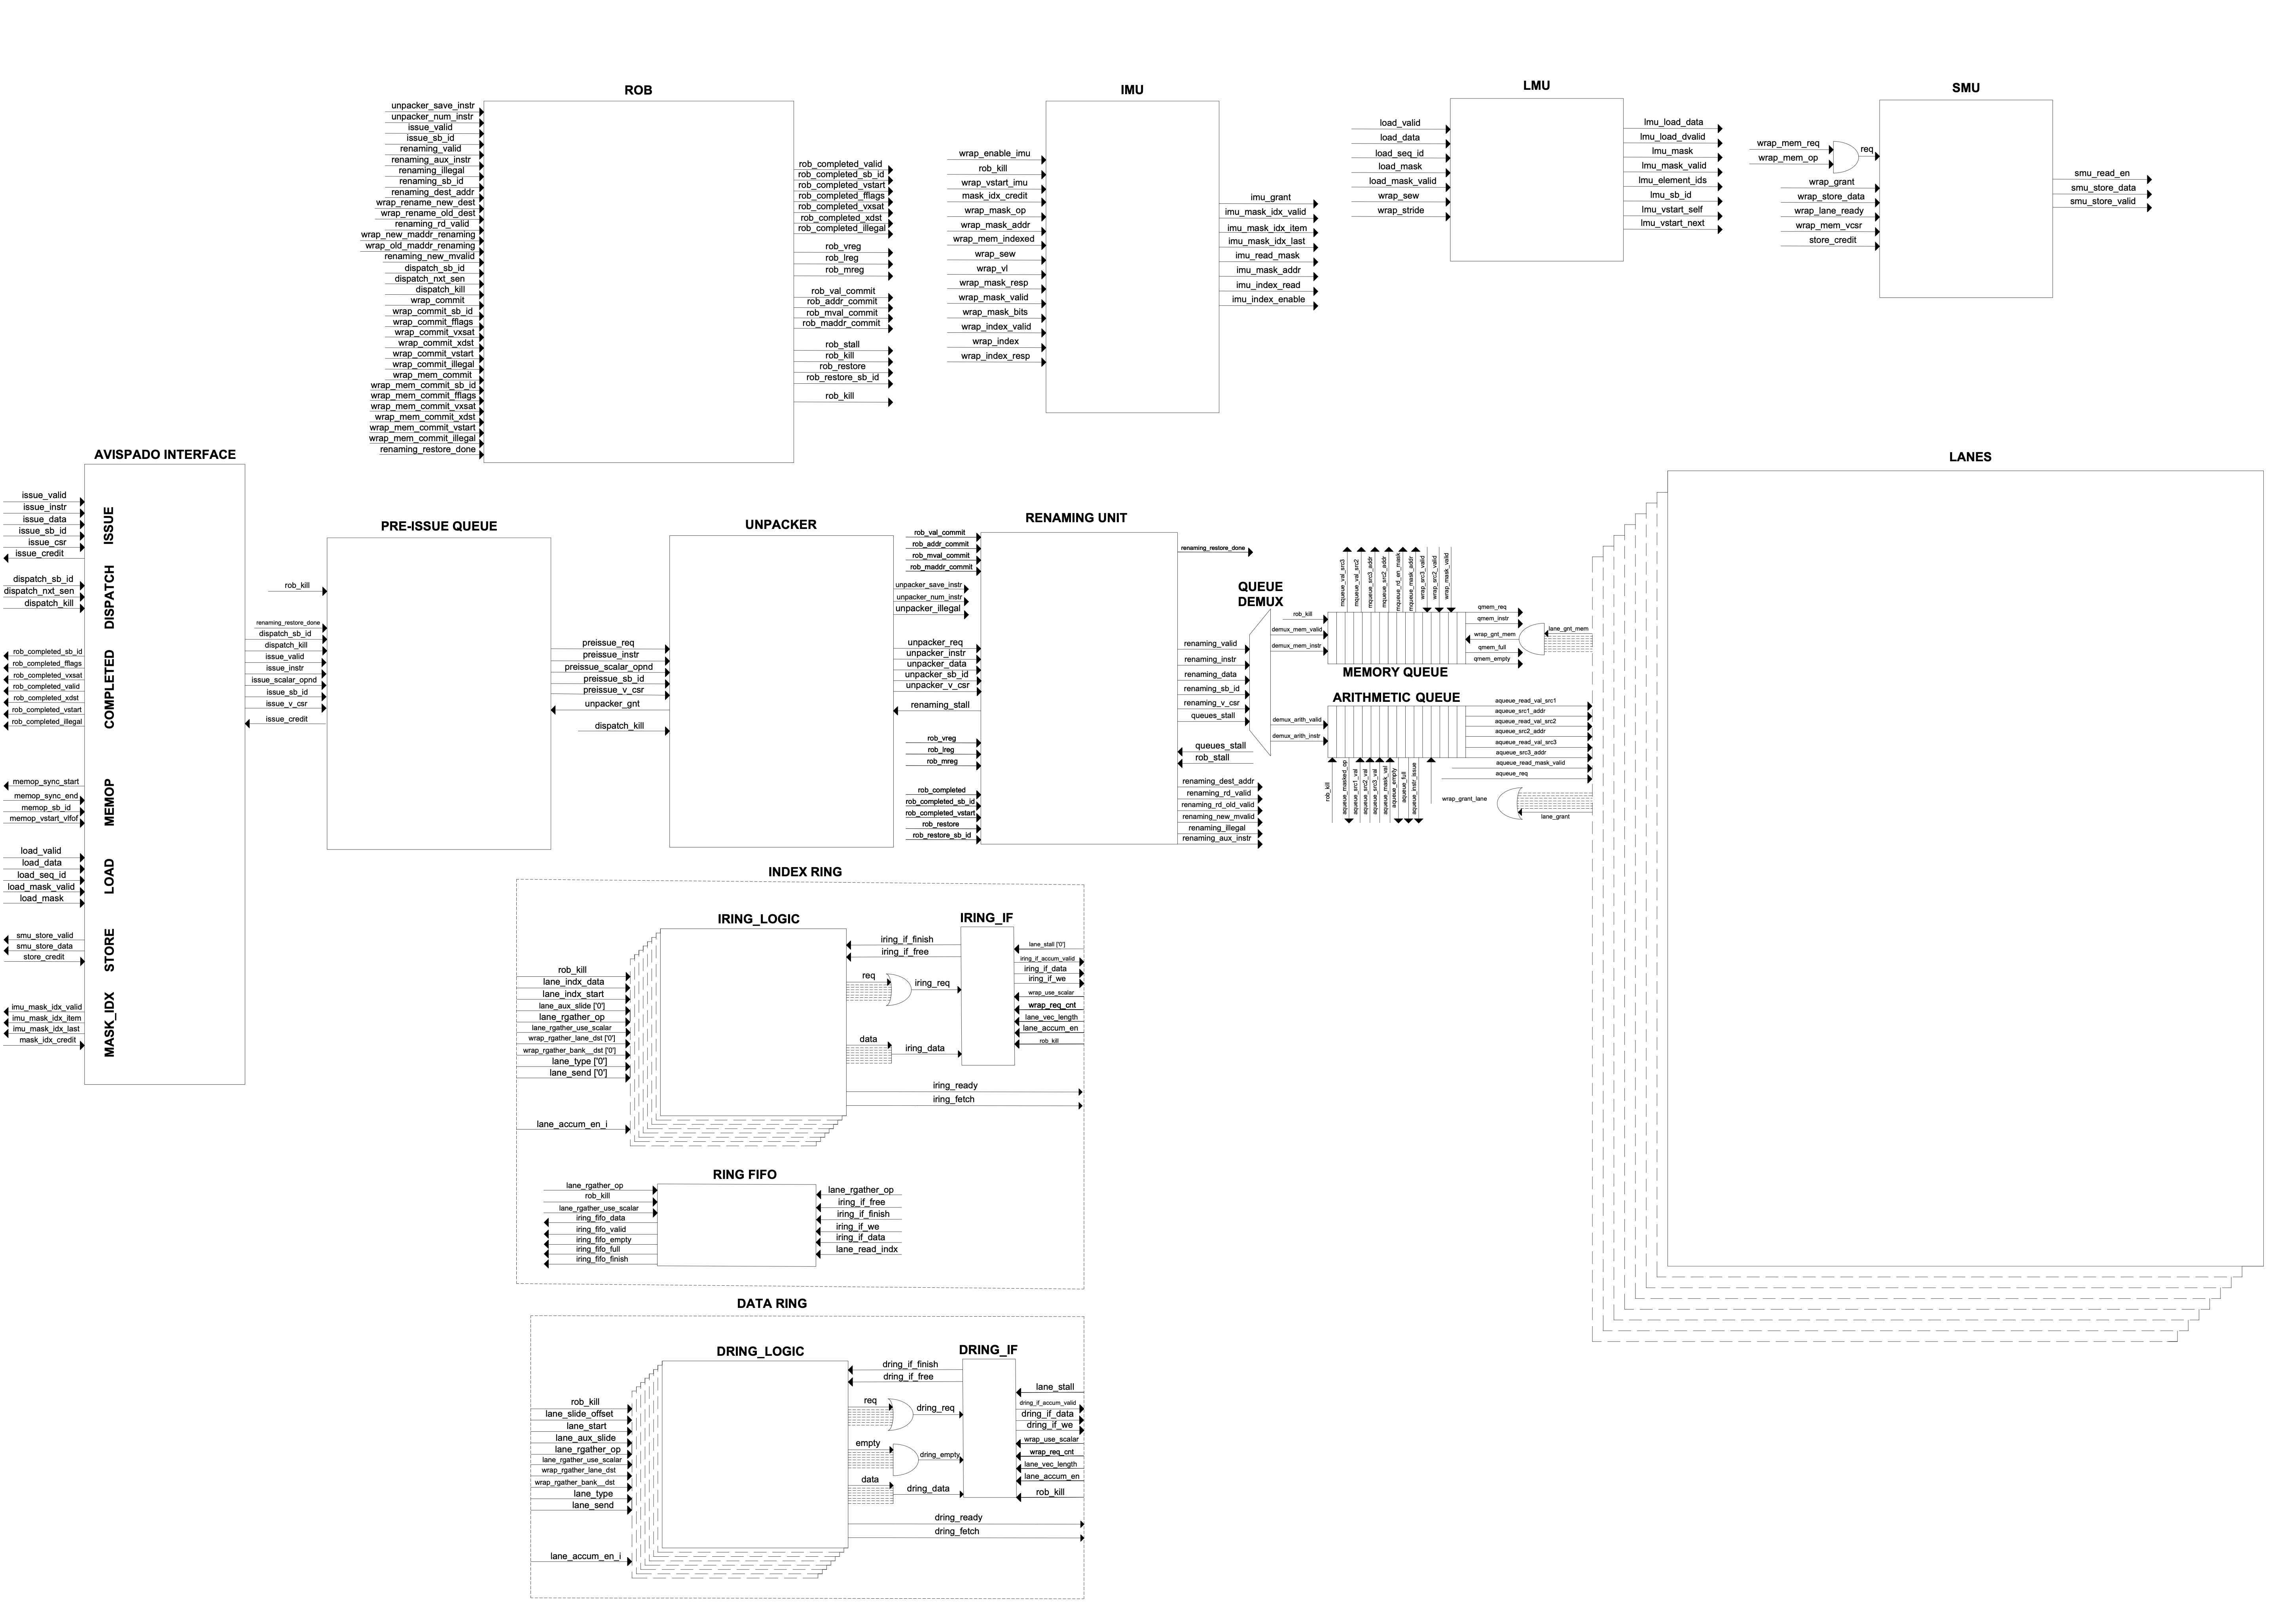
\includegraphics[scale = 0.07]{Chapter_1/img/VPU-wo-LANE.jpg}
    \caption{EPI project's VPU}
    \label{VPU-wo-LANE}
\end{figure}
%%images by victor, take the google drive infos

\subsection{Submodules}
%description on LB and LMU mainly and on the checkers in generale

\subsection{The UVM and the checkers}
%%the all draw in to the wiki and the main description of every piece would be great.


\include{The_work/The_work}
\include{Contributions/Contributions}
\include{Conclusions/Conclusions}



\begin{appendix}
  \listoffigures
  \listoftables
\end{appendix}

\newpage

\bibliographystyle{plain}
\bibliography{mybib}

%nocite{*}




\end{document}






\end{document}
